% Отчёт по этапу 2 курсовой работы. Компилируется xelatex.
\documentclass[12pt,a4paper]{article}
\usepackage{fontspec}
\IfFontExistsTF{Times New Roman}{\setmainfont{Times New Roman}}{\setmainfont{Liberation Serif}}
\IfFontExistsTF{Courier New}{\setmonofont{Courier New}}{%
  \IfFontExistsTF{Liberation Mono}{\setmonofont{Liberation Mono}}{\setmonofont{DejaVu Sans Mono}}}
\IfFileExists{polyglossia.sty}{\usepackage{polyglossia}\setdefaultlanguage{russian}}{\usepackage[russian]{babel}}

\usepackage[left=25mm,right=15mm,top=20mm,bottom=20mm]{geometry}
\usepackage{longtable,array,booktabs,graphicx,caption,enumitem,xcolor}
\usepackage{listings}
\usepackage[unicode,hidelinks]{hyperref}
\setlist{nosep}
\setlength{\emergencystretch}{2em}
\captionsetup{labelsep=endash}
\captionsetup[table]{name=Таблица,justification=raggedright,singlelinecheck=false}
\newcolumntype{L}[1]{>{\raggedright\arraybackslash}p{#1}}
\graphicspath{{../img/}}

\lstdefinestyle{sql}{language=SQL, basicstyle=\ttfamily\scriptsize, columns=fullflexible,
  keepspaces=true, breaklines=true, extendedchars=true,
  frame=single, framerule=0.3pt, rulecolor=\color{gray},
  keywordstyle=\bfseries, commentstyle=\color{gray}\itshape,
  morekeywords={RETURNS,LANGUAGE,TRIGGER,PROCEDURE,CALL,PERFORM,RAISE,EXCEPTION,
    LOOP,EXIT,IF,ELSIF,THEN,END,DECLARE,BEGIN,RETURN,QUERY,RETURNING,ENUM,TYPE,
    REFERENCES,RESTRICT,CASCADE,INCLUDE,BOOLEAN,TEXT,SERIAL,BIGSERIAL,SMALLSERIAL,
    TIMESTAMPTZ,JSONB,COMMENT,EXECUTE,FUNCTION,FOUND,STABLE,IMMUTABLE}}
\lstset{style=sql}

\begin{document}

\begin{titlepage}
\centering
Университет ИТМО\\
Факультет программной инженерии и компьютерной техники

\vspace{60mm}
{\Large\bfseries Курсовая работа\par}
\vspace{4mm}
{\large Этап 2. Модель данных и её реализация в PostgreSQL\par}
\vspace{8mm}
{\large Информационная система «Бдительность»\par}

\vfill
\begin{flushright}
Выполнил: студент группы P3310\\
Мыц Иван Евгеньевич
\end{flushright}
\vspace{20mm}
Санкт-Петербург, 2026
\end{titlepage}

\section{ER-модель}
\begin{center}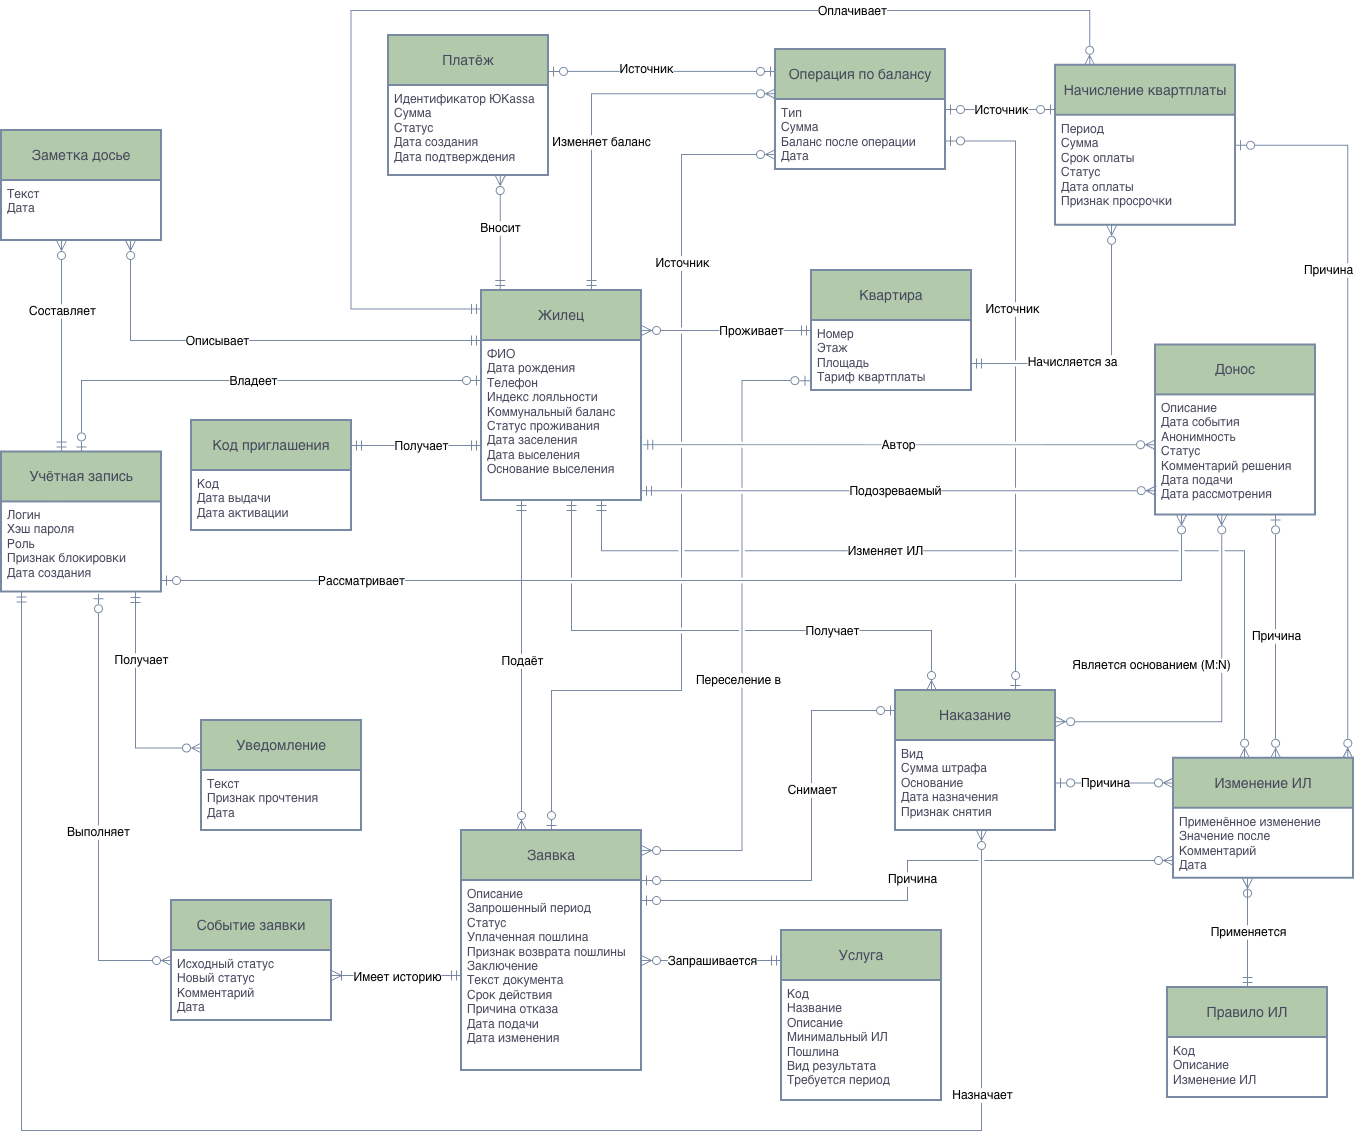
\includegraphics[width=\textwidth]{er_model.png}\end{center}
\begin{longtable}{L{35.3mm} L{51.0mm} L{70.6mm}}
\caption{Сущности}\label{tab:ent}\\
\toprule \textbf{Сущность} & \textbf{Описание} & \textbf{Атрибуты} \\ \midrule
\endfirsthead
\toprule \textbf{Сущность} & \textbf{Описание} & \textbf{Атрибуты} \\ \midrule
\endhead
\bottomrule
\endfoot
Учётная запись & Данные для входа жильца или управляющего. & логин, хеш пароля, роль, признак блокировки, дата создания \\
Жилец & Человек, проживающий в доме. & ФИО, дата рождения, телефон, индекс лояльности, коммунальный баланс, статус проживания, даты заселения и выселения, основание выселения \\
Код приглашения & Одноразовый код для активации учётной записи. & код, дата выдачи, дата активации \\
Квартира & Квартира дома, в ней живёт до 10 жильцов. & номер, этаж, площадь, тариф квартплаты \\
Услуга & Услуга из фиксированного перечня SV01--SV09. & код, название, описание, минимальный ИЛ, пошлина, вид результата, требуется период \\
Заявка & Обращение жильца за услугой и его результат. & описание, запрошенный период, статус, уплаченная пошлина, признак возврата пошлины, заключение, текст документа, срок действия, причина отказа, даты подачи и изменения \\
Событие заявки & Запись истории обработки заявки. & исходный статус, новый статус, комментарий, дата \\
Донос & Сообщение жильца о нарушении соседа. & описание, дата события, анонимность, статус, комментарий решения, даты подачи и рассмотрения \\
Наказание & Предупреждение, штраф или выселение. & вид, сумма штрафа, основание, дата назначения, признак снятия \\
Платёж & Пополнение баланса через ЮKassa. & идентификатор ЮKassa, сумма, статус, даты создания и подтверждения \\
Начисление квартплаты & Ежемесячное начисление за квартиру; оплачивает любой её жилец. & период, сумма, срок оплаты, статус, дата оплаты, признак просрочки \\
Операция по балансу & Запись журнала изменений баланса. & тип, сумма, баланс после операции, дата \\
Правило ИЛ & Правило изменения ИЛ RL01--RL07. & код, описание, изменение ИЛ \\
Изменение ИЛ & Запись журнала изменений ИЛ. & применённое изменение, значение после, комментарий, дата \\
Заметка досье & Наблюдение управляющего о жильце. & текст, дата \\
Уведомление & Сообщение пользователю о событии. & текст, признак прочтения, дата \\
\end{longtable}
\begin{longtable}{L{49.0mm} L{23.5mm} L{84.3mm}}
\caption{Связи}\label{tab:rel}\\
\toprule \textbf{Связь} & \textbf{Тип связи} & \textbf{Пояснение} \\ \midrule
\endfirsthead
\toprule \textbf{Связь} & \textbf{Тип связи} & \textbf{Пояснение} \\ \midrule
\endhead
\bottomrule
\endfoot
Учётная запись — Жилец & 0..1 : 0..1 & Учётная запись появляется после активации кода; у управляющего записи жильца нет. \\
Учётная запись — Уведомление & 1 : 0..* & Пользователь получает уведомления. \\
Учётная запись — Заметка досье & 1 : 0..* & Управляющий составляет заметку. \\
Жилец — Заметка досье & 1 : 0..* & Заметка описывает жильца. \\
Жилец — Код приглашения & 1 : 1 & При заселении жильцу выдаётся код. \\
Жилец — Квартира & 0..* : 1 & Жилец проживает в квартире; одновременно в квартире живут до 10 жильцов. \\
Жилец — Донос & 1 : 0..* & Жилец — автор доноса. \\
Жилец — Донос & 1 : 0..* & Жилец — подозреваемый по доносу. \\
Учётная запись — Донос & 0..1 : 0..* & Управляющий рассматривает донос. \\
Жилец — Заявка & 1 : 0..* & Жилец подаёт заявки. \\
Услуга — Заявка & 1 : 0..* & Заявка подаётся на одну услугу. \\
Квартира — Заявка & 0..1 : 0..* & Квартира для переселения (SV07). \\
Заявка — Событие заявки & 1 : 1..* & Заявка имеет историю обработки. \\
Учётная запись — Событие заявки & 0..1 : 0..* & Пользователь, изменивший статус. \\
Жилец — Наказание & 1 : 0..* & Жилец получает наказание. \\
Учётная запись — Наказание & 1 : 0..* & Управляющий назначает наказание. \\
\textbf{Донос — Наказание} & \textbf{0..* : 0..*} & \textbf{Наказание назначается по одному или нескольким доносам; по доносу может быть назначено несколько наказаний.} \\
Заявка — Наказание & 0..1 : 0..1 & Заявка SV09 снимает предупреждение. \\
Жилец — Платёж & 1 : 0..* & Жилец вносит платёж. \\
Жилец — Начисление квартплаты & 0..1 : 0..* & Начисление оплачивает один из жильцов квартиры. \\
Квартира — Начисление квартплаты & 1 : 0..* & Квартплата начисляется за квартиру. \\
Жилец — Операция по балансу & 1 : 0..* & Операция изменяет баланс жильца. \\
Платёж, Начисление, Заявка, Наказание — Операция по балансу & 0..1 : 0..1 & Источник операции (для заявки 0..1 : 0..*: пошлина и её возврат). \\
Жилец — Изменение ИЛ & 1 : 0..* & Изменение ИЛ жильца. \\
Правило ИЛ — Изменение ИЛ & 1 : 0..* & Изменение выполняется по правилу. \\
Донос, Наказание, Начисление, Заявка — Изменение ИЛ & 0..1 : 0..* & Причина изменения ИЛ. \\
\end{longtable}
\textbf{УДАЛИТЬ} Связь «многие-ко-многим» здесь одна --- «Донос — Наказание». Пример из тестовых данных: штраф Мельнику назначен сразу по трём доносам, а Ершову по одному доносу назначены и штраф, и предупреждение. «Учётная запись — Жилец» необязательна с обеих сторон: жилец существует до активации кода, а у управляющего есть учётная запись, но нет записи жильца. «Заявка — Наказание»: выполнение услуги SV09 «Снятие предупреждения» помечает последнее действующее предупреждение снятым, само наказание не удаляется. «Операция по балансу» и «Изменение ИЛ» --- журналы: баланс и ИЛ жильца всегда равны сумме записей журнала, записи не изменяются и не удаляются. \textbf{УДАЛИТЬ}
\section{Даталогическая модель}
\begin{center}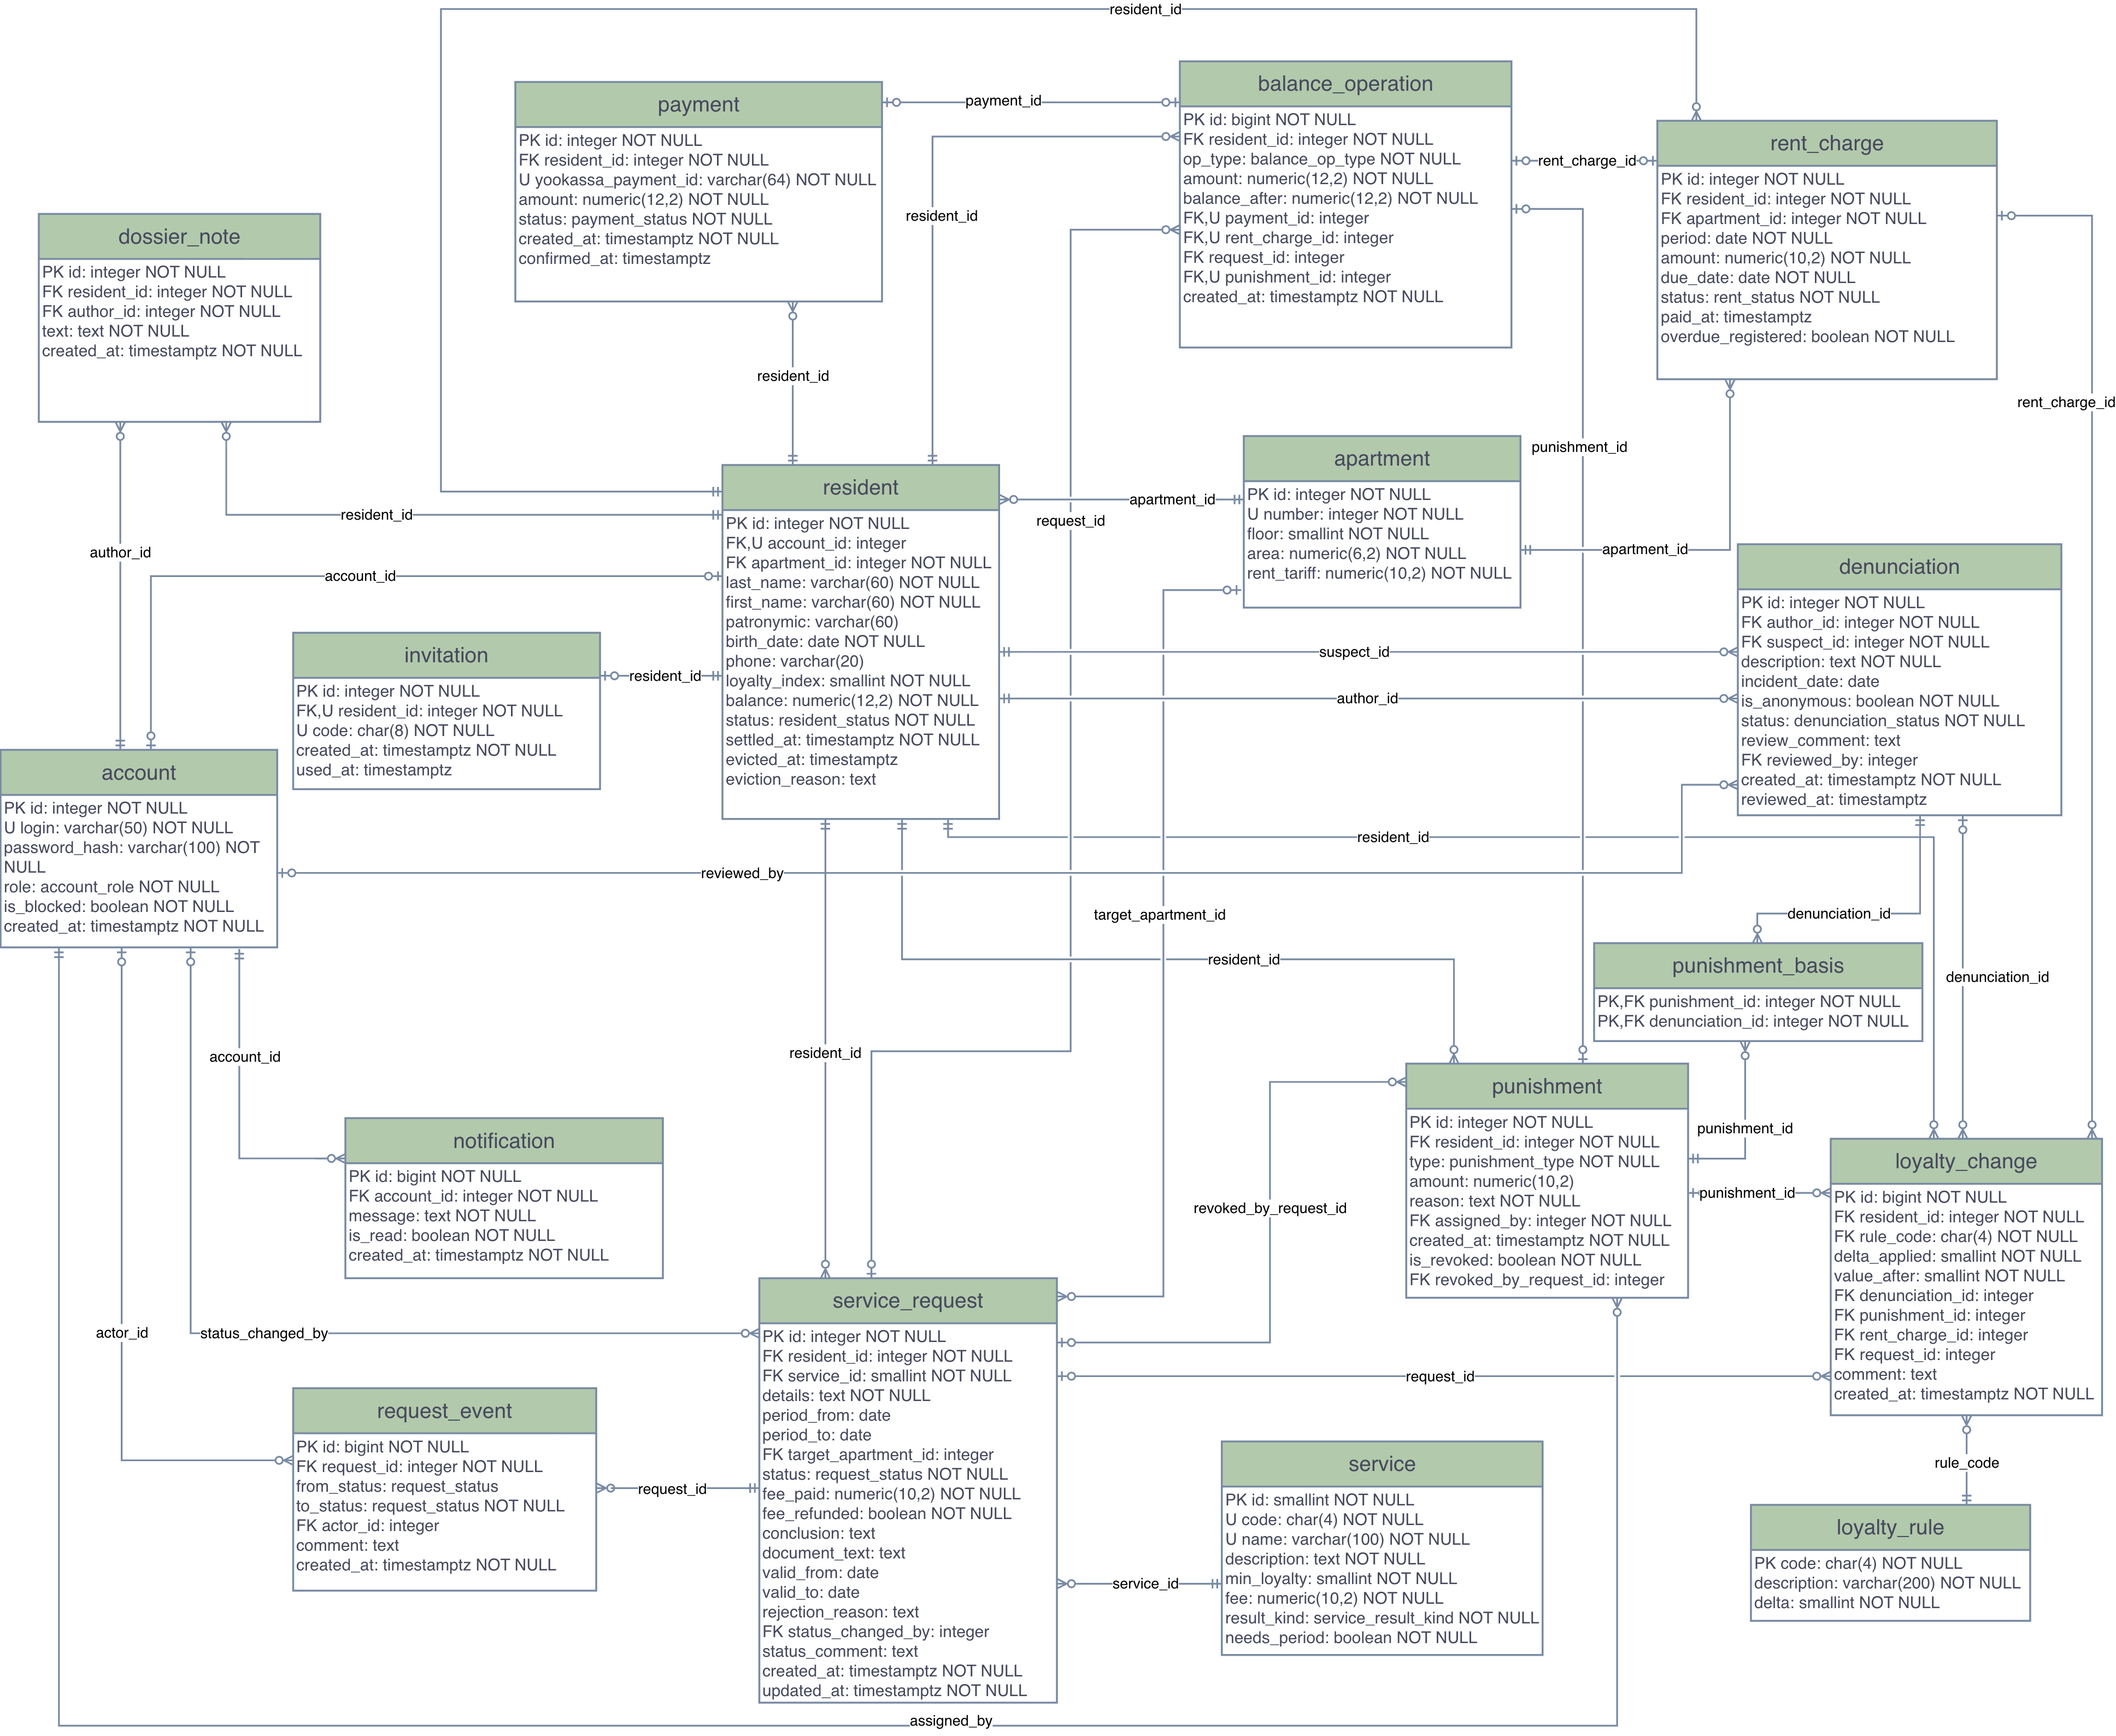
\includegraphics[width=\textwidth]{datalogical_model.png}\end{center}
\begin{longtable}{L{30.5mm} L{31.4mm} L{35.2mm} L{55.2mm}}
\caption{Первичные и внешние ключи}\label{tab:keys}\\
\toprule \textbf{Таблица} & \textbf{Сущность} & \textbf{Первичный ключ} & \textbf{Внешние ключи} \\ \midrule
\endfirsthead
\toprule \textbf{Таблица} & \textbf{Сущность} & \textbf{Первичный ключ} & \textbf{Внешние ключи} \\ \midrule
\endhead
\bottomrule
\endfoot
\texttt{account} & Учётная запись & \texttt{id} & — \\
\texttt{resident} & Жилец & \texttt{id} & \texttt{account\_\allowbreak{}id (U), apartment\_\allowbreak{}id} \\
\texttt{invitation} & Код приглашения & \texttt{id} & \texttt{resident\_\allowbreak{}id (U)} \\
\texttt{apartment} & Квартира & \texttt{id} & — \\
\texttt{service} & Услуга & \texttt{id} & — \\
\texttt{service\_\allowbreak{}request} & Заявка & \texttt{id} & \texttt{resident\_\allowbreak{}id, service\_\allowbreak{}id, target\_\allowbreak{}apartment\_\allowbreak{}id, status\_\allowbreak{}changed\_\allowbreak{}by} \\
\texttt{request\_\allowbreak{}event} & Событие заявки & \texttt{id} & \texttt{request\_\allowbreak{}id, actor\_\allowbreak{}id} \\
\texttt{denunciation} & Донос & \texttt{id} & \texttt{author\_\allowbreak{}id, suspect\_\allowbreak{}id, reviewed\_\allowbreak{}by} \\
\texttt{punishment} & Наказание & \texttt{id} & \texttt{resident\_\allowbreak{}id, assigned\_\allowbreak{}by, revoked\_\allowbreak{}by\_\allowbreak{}request\_\allowbreak{}id} \\
\texttt{punishment\_\allowbreak{}basis} & Связь M:N «Донос — Наказание» & \texttt{(punishment\_\allowbreak{}id, denunciation\_\allowbreak{}id)} & \texttt{punishment\_\allowbreak{}id, denunciation\_\allowbreak{}id} \\
\texttt{payment} & Платёж & \texttt{id} & \texttt{resident\_\allowbreak{}id} \\
\texttt{rent\_\allowbreak{}charge} & Начисление квартплаты & \texttt{id} & \texttt{apartment\_\allowbreak{}id, paid\_\allowbreak{}by} \\
\texttt{balance\_\allowbreak{}operation} & Операция по балансу & \texttt{id} & \texttt{resident\_\allowbreak{}id, payment\_\allowbreak{}id (U), rent\_\allowbreak{}charge\_\allowbreak{}id (U), request\_\allowbreak{}id, punishment\_\allowbreak{}id (U)} \\
\texttt{loyalty\_\allowbreak{}rule} & Правило ИЛ & \texttt{code} & — \\
\texttt{loyalty\_\allowbreak{}change} & Изменение ИЛ & \texttt{id} & \texttt{resident\_\allowbreak{}id, rule\_\allowbreak{}code, denunciation\_\allowbreak{}id, punishment\_\allowbreak{}id, rent\_\allowbreak{}charge\_\allowbreak{}id, request\_\allowbreak{}id} \\
\texttt{dossier\_\allowbreak{}note} & Заметка досье & \texttt{id} & \texttt{resident\_\allowbreak{}id, author\_\allowbreak{}id} \\
\texttt{notification} & Уведомление & \texttt{id} & \texttt{account\_\allowbreak{}id} \\
\end{longtable}
Все таблицы находятся в третьей нормальной форме: значения атрибутов атомарны, каждый
неключевой атрибут зависит от всего первичного ключа и не зависит от других неключевых атрибутов.

\textbf{УДАЛИТЬ} Если спросят про \texttt{resident.\allowbreak{}balance} и \texttt{resident.\allowbreak{}loyalty\_\allowbreak{}index}: это не нарушение 3НФ. Нормальные формы описывают зависимости внутри одной таблицы, а эти столбцы зависят только от \texttt{id} жильца. Они совпадают с суммами журналов \texttt{balance\_\allowbreak{}operation} и \texttt{loyalty\_\allowbreak{}change} и хранятся, чтобы быстро проверять условия подачи заявок и сортировать очередь. Совпадение гарантируют триггеры: напрямую изменить баланс или ИЛ нельзя. \texttt{service\_\allowbreak{}request.\allowbreak{}fee\_\allowbreak{}paid} и \texttt{rent\_\allowbreak{}charge.\allowbreak{}amount} --- не копии \texttt{service.\allowbreak{}fee} и \texttt{apartment.\allowbreak{}rent\_\allowbreak{}tariff}, а значения на момент операции: тариф может измениться, а история --- нет. Отрицательный баланс означает задолженность по штрафам, поэтому отдельного поля для долга нет. \textbf{УДАЛИТЬ}
\section{Реализация в PostgreSQL}
Модель реализована набором SQL-скриптов (таблица~\ref{tab:scripts}).

\begin{longtable}{L{38.3mm} L{122.9mm}}
\caption{Скрипты}\label{tab:scripts}\\
\toprule \textbf{Файл} & \textbf{Назначение} \\ \midrule
\endfirsthead
\toprule \textbf{Файл} & \textbf{Назначение} \\ \midrule
\endhead
\bottomrule
\endfoot
\texttt{install.\allowbreak{}sql} & Создание базы целиком: выполняет скрипты 01--04. \\
\texttt{00\_\allowbreak{}drop.sql} & Удаление всех объектов базы. \\
\texttt{01\_\allowbreak{}create.sql} & Типы, таблицы, ограничения, справочники услуг и правил ИЛ. \\
\texttt{02\_\allowbreak{}triggers.sql} & Триггеры. \\
\texttt{03\_\allowbreak{}functions.sql} & Функции для критически важных запросов и представления. \\
\texttt{04\_\allowbreak{}indexes.sql} & Индексы. \\
\texttt{05\_\allowbreak{}fill.sql} & Тестовые данные: 30 квартир, 24 жильца, заявки во всех статусах, доносы, наказания. \\
\texttt{06\_\allowbreak{}fill\_\allowbreak{}bulk.sql} & Массовые данные для проверки индексов: 300 жильцов, 10\,000 заявок и 10\,000 доносов. \\
\texttt{tests/} & Тесты базы на Java (JUnit 5, JDBC): 14 тестов в двух классах, запуск 	exttt{mvn test}. \\
\end{longtable}
\begin{lstlisting}[language=bash]
psql -h pg -d studs -f install.sql
psql -h pg -d studs -f 05_fill.sql
cd tests && mvn test
\end{lstlisting}

\textbf{УДАЛИТЬ} Тесты проверяют ограничения таблиц, журналы баланса и ИЛ, вместимость квартиры, модели состояний заявки и доноса, связь M:N и каждую функцию. Каждый тест сам создаёт нужные строки в своей транзакции и откатывает её, поэтому тесты проходят и на пустой, и на заполненной базе. Ошибки проверяются по коду SQLSTATE. \textbf{УДАЛИТЬ}

\textbf{УДАЛИТЬ} На helios нельзя выполнить \texttt{CREATE DATABASE}, поэтому скрипты создают объекты в личной схеме базы \texttt{studs}. Нужен PostgreSQL 11 или новее. Целостность обеспечена ограничениями \texttt{NOT NULL}, \texttt{CHECK}, \texttt{UNIQUE}, внешними ключами и 10 триггерами --- их описание в файле с вопросами к защите и в листинге \texttt{02\_\allowbreak{}triggers.sql}. Триггеры защищают только данные: журналы, согласованность баланса и ИЛ с журналами, вместимость квартиры (до 10 жильцов), модели состояний и историю заявок. Пароли тестовых пользователей: \texttt{manager/manager123}, жильцы \texttt{/resident123}. \textbf{УДАЛИТЬ}
\section{Функции}
Бизнес-логику реализует серверная часть на Spring, простые чтения и изменения она выполняет
через ORM. Функции предложены для критически важных запросов: операций, которые должны
выполняться атомарно, и выборок, которые удобнее выполнить одним запросом (таблица~\ref{tab:fn}).
Представление \texttt{v\_\allowbreak{}denunciation\_\allowbreak{}for\_\allowbreak{}manager} скрывает автора анонимного доноса,
\texttt{v\_\allowbreak{}loyalty\_\allowbreak{}history} --- ссылки на доносы в истории ИЛ.

\begin{longtable}{L{45.1mm} L{21.6mm} L{90.2mm}}
\caption{Функции}\label{tab:fn}\\
\toprule \textbf{Имя} & \textbf{Где используется} & \textbf{Что делает} \\ \midrule
\endfirsthead
\toprule \textbf{Имя} & \textbf{Где используется} & \textbf{Что делает} \\ \midrule
\endhead
\bottomrule
\endfoot
\texttt{activate\_\allowbreak{}account} & UC01 & Помечает код приглашения использованным, создаёт учётную запись и привязывает её к жильцу. \\
\texttt{apply\_\allowbreak{}payment\_\allowbreak{}status} & UC04 & Применяет статус платежа из ЮKassa и зачисляет деньги ровно один раз. \\
\texttt{pay\_\allowbreak{}rent} & UC06 & Отмечает начисление квартиры оплаченным жильцом и списывает сумму с его баланса; повторно оплатить нельзя. \\
\texttt{accrue\_\allowbreak{}rent} & S001 & Начисляет квартплату за месяц одним запросом: одно начисление на квартиру с жильцами. \\
\texttt{register\_\allowbreak{}overdue\_\allowbreak{}rent} & S002 & Отмечает просроченные начисления и возвращает жильцов этих квартир. \\
\texttt{request\_\allowbreak{}queue} & UC17 & Возвращает очередь необработанных заявок по убыванию ИЛ заявителей. \\
\texttt{resident\_\allowbreak{}dossier} & UC15 & Возвращает досье жильца одним документом JSON без авторов анонимных доносов. \\
\end{longtable}
\textbf{УДАЛИТЬ} Почему именно эти функции: активация, зачисление платежа и оплата квартплаты меняют несколько таблиц и должны выполняться целиком или не выполняться вовсе; повторный вызов \texttt{apply\_\allowbreak{}payment\_\allowbreak{}status} ничего не меняет, поэтому опрос ЮKassa безопасен. Начисление и просрочка квартплаты обрабатывают всех жильцов одним запросом. Очередь заявок и досье --- выборки из многих таблиц, которые удобно получить одним вызовом. Остальные прецеденты --- обычные чтения и изменения через ORM: условия подачи заявок, правила ИЛ, уведомления, последствия наказаний и права пользователей проверяет Spring. Ошибки имеют коды SQLSTATE: BH404 --- не найдено, BH409 --- недопустимо в текущем состоянии, BH422 --- не выполнено условие; Spring по коду выбирает ответ HTTP. \textbf{УДАЛИТЬ}
\section{Индексы}
Индексы созданы для запросов, которые выполняются при каждом открытии страниц кабинета
(таблица~\ref{tab:ix}). Индексы первичных ключей и ограничений \texttt{UNIQUE} PostgreSQL создаёт сам.

\begin{longtable}{L{8.3mm} L{42.6mm} L{48.1mm} L{13.0mm} L{36.1mm}}
\caption{Индексы}\label{tab:ix}\\
\toprule \textbf{№} & \textbf{Индекс} & \textbf{Столбцы} & \textbf{UC} & \textbf{Где используется} \\ \midrule
\endfirsthead
\toprule \textbf{№} & \textbf{Индекс} & \textbf{Столбцы} & \textbf{UC} & \textbf{Где используется} \\ \midrule
\endhead
\bottomrule
\endfoot
I1 & \texttt{idx\_\allowbreak{}request\_\allowbreak{}active} & \texttt{service\_\allowbreak{}request (status, created\_\allowbreak{}at)}, только необработанные заявки & UC17 & Очередь заявок (\texttt{request\_\allowbreak{}queue}) \\
I2 & \texttt{idx\_\allowbreak{}request\_\allowbreak{}resident} & \texttt{service\_\allowbreak{}request (resident\_\allowbreak{}id, created\_\allowbreak{}at)} & UC10 & Список заявок жильца \\
I3 & \texttt{idx\_\allowbreak{}request\_\allowbreak{}event\_\allowbreak{}request} & \texttt{request\_\allowbreak{}event (request\_\allowbreak{}id, created\_\allowbreak{}at)} & UC10 & История обработки заявки \\
I4 & \texttt{idx\_\allowbreak{}denunciation\_\allowbreak{}pending} & \texttt{denunciation (created\_\allowbreak{}at)}, только нерассмотренные доносы & UC22 & Очередь доносов \\
I5 & \texttt{idx\_\allowbreak{}balance\_\allowbreak{}operation\_\allowbreak{}resident} & \texttt{balance\_\allowbreak{}operation (resident\_\allowbreak{}id, created\_\allowbreak{}at)} & UC05 & История операций по балансу \\
I6 & \texttt{idx\_\allowbreak{}notification\_\allowbreak{}unread} & \texttt{notification (account\_\allowbreak{}id, created\_\allowbreak{}at)}, только непрочитанные & U019 & Непрочитанные уведомления \\
\end{longtable}
\textbf{УДАЛИТЬ} Индексы I1, I4 и I6 частичные (\texttt{WHERE}): в них попадают только «активные» строки, поэтому они маленькие и не растут вместе с историей. Индексы по внешним ключам PostgreSQL автоматически не создаёт, поэтому без I2, I3 и I5 запрос «все записи жильца» читает всю таблицу. Запросы для I2--I6 приложение выполняет через ORM, индекс используется независимо от того, кто сформировал запрос. \textbf{УДАЛИТЬ}
\subsection{Проверка}
Индексы проверены на массовых данных (\texttt{06\_\allowbreak{}fill\_\allowbreak{}bulk.sql}: 300 жильцов, 10\,013 заявок, 28\,434 записей
истории заявок, 10\,023 доносов, 18\,568 уведомлений). Для каждого запроса выполнена команда \texttt{EXPLAIN ANALYZE}
без индексов и с ними (таблица~\ref{tab:explain}).

\begin{longtable}{L{34.8mm} L{9.7mm} L{25.1mm} L{13.5mm} L{29.0mm} L{13.5mm} L{13.5mm}}
\caption{Время выполнения запросов}\label{tab:explain}\\
\toprule \textbf{Запрос} & \textbf{Инд.} & \textbf{Без индекса} & \textbf{мс} & \textbf{С индексом} & \textbf{мс} & \textbf{Уск.} \\ \midrule
\endfirsthead
\toprule \textbf{Запрос} & \textbf{Инд.} & \textbf{Без индекса} & \textbf{мс} & \textbf{С индексом} & \textbf{мс} & \textbf{Уск.} \\ \midrule
\endhead
\bottomrule
\endfoot
Очередь заявок & I1 & Seq Scan & 2.73 & Bitmap Index Scan & 1.57 & 1.7\,$\times$ \\
Заявки жильца & I2 & Seq Scan & 1.11 & Index Scan & 0.11 & 10\,$\times$ \\
История заявки & I3 & Seq Scan & 1.41 & Bitmap Index Scan & 0.13 & 11\,$\times$ \\
Очередь доносов & I4 & Seq Scan & 0.90 & Index Scan & 0.07 & 14\,$\times$ \\
Операции по балансу & I5 & Seq Scan & 0.44 & Bitmap Index Scan & 0.17 & 3\,$\times$ \\
Непрочитанные уведомления & I6 & Seq Scan & 1.21 & Index Scan & 0.07 & 16\,$\times$ \\
\end{longtable}
Без индексов каждый запрос читает всю таблицу (\texttt{Seq Scan}), с индексами --- только нужные
строки. Сильнее всего ускорились выборки нескольких строк из больших таблиц: история заявки,
непрочитанные уведомления, заявки жильца.

\textbf{УДАЛИТЬ} Очередь заявок (I1) ускоряется слабо: в результат попадают все необработанные заявки, и они сортируются по ИЛ заявителя из другой таблицы. Индекс полезен тем, что объём чтения не зависит от числа уже выполненных заявок, которые копятся годами. \textbf{УДАЛИТЬ}
\section{Заключение}
Построены ER-модель из 16 сущностей со связью «многие-ко-многим» и даталогическая модель из 17 таблиц.
Модель реализована в PostgreSQL вместе с ограничениями целостности, триггерами, функциями для
критически важных запросов и индексами; написаны скрипты создания, удаления и заполнения базы.

\newpage
\section*{Приложение А. Листинги скриптов}
\addcontentsline{toc}{section}{Приложение А. Листинги скриптов}
\subsection*{01\_\allowbreak{}create.sql}
\lstinputlisting{../sql/01_create.sql}
\subsection*{02\_\allowbreak{}triggers.sql}
\lstinputlisting{../sql/02_triggers.sql}
\subsection*{03\_\allowbreak{}functions.sql}
\lstinputlisting{../sql/03_functions.sql}
\subsection*{04\_\allowbreak{}indexes.sql}
\lstinputlisting{../sql/04_indexes.sql}

\end{document}
